\documentclass{beamer}
%\usepackage[utf8]{vietnam}
\usepackage[vietnamese]{babel}
\usepackage{hyperref}
\usepackage{graphicx}
\usepackage{lmodern}
\usepackage{tikz}
\usepackage{calc}

\graphicspath{{./images/}}
\usetheme{Antibes}
\title{Deep Factorization Machines}
\author{Đỗ Hoàng Thuấn}
\date{Octorber 2019}
 
\begin{document}

\frame{\titlepage}

\begin{frame}
\frametitle{Table of contents}
\tableofcontents
\end{frame}

\section{Introduction}
\begin{frame}
	\frametitle{Introduction}
	\begin{itemize}
 		\item Deep factorization machine is SOTA in Click Through Rate problem.
 		\item DeepFM makes a good result on Zalo Hit Song Challenge.
	\end{itemize}
\end{frame}

\section{Factorization Machine}
\frame{\tableofcontents[currentsection]}
\begin{frame}
	\frametitle{Problem statement}
	Deep FM is build based on FM. \\
	Suppose we have a dataset. \\
	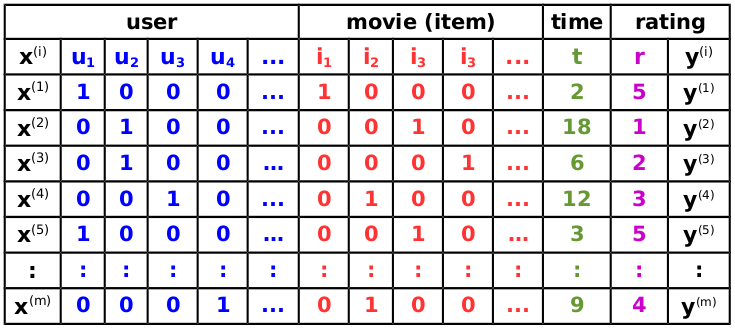
\includegraphics[scale=0.35]{data} \\
	where:
	\begin{itemize}
		\item X $\in R^{m \times n}$ 
		\item m is number of observations, $n = n_{user} + n_{item} + n_T$ 
		\item $x$ is feature vector, $v \int$
	\end{itemize}
\end{frame}

\begin{frame}
	\frametitle{Result of FM}
	\begin{figure}
		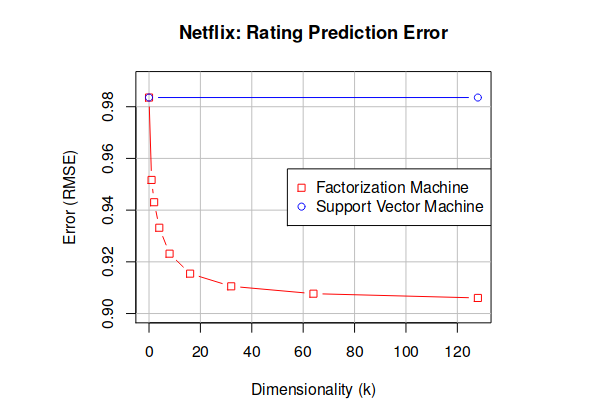
\includegraphics[scale=0.5]{fm_result}
	\end{figure}
\end{frame}

\begin{frame}
	\frametitle{Polynomial model and limitation}
	Apply polynomial( linear regresson).
	\begin{equation}
		\sigma = w_{0} + \sum_{i=1}^{n} w_{i} x_{i} 
	\end{equation}
	where:
	\begin{description}
		\item[$w_0$] is bias
		\item[$w_i$] is weight of field i
		\item[$x_i$] is feature vector of field i 	
	\end{description}	
	Polynomial does not use combination of features. \\
	Can not get the interaction between features.
\end{frame}

\begin{frame}
	\frametitle{Factorization Machine}
	Extends from logistic regression. \\
	Equation of 2-order FM. \\
	\[
	\hat{y}(x) = w_{0} + \sum_{i=1}^{i=n} w_{i} x_{i} + \sum_{i=1}^n \sum_{j=i+1}^n<v_i, v_j>x_i x_j
	\]
	Where: 
	\begin{description}
		\item[$w_0$] is bias
		\item[$w_i$] is weight of field i.
		\item[$x_i$] is feature vector of field i. 
		\item[$v$] is latent feature vector.
		\item[$\hat{w}_{i,j} =n<v_i, v_j>$] is interaction between the i-th and j-th variable.
	\end{description}
\end{frame}
\section{Deep Factorization Machine}
\frame{\tableofcontents[currentsection]}
\subsection{Introduction to Deep Factorization Machine}
\begin{frame}	
	\frametitle{Factorization Machine Layer}	
	Intergrate the architecture of FM and deep neural networks.	
	\begin{figure}
		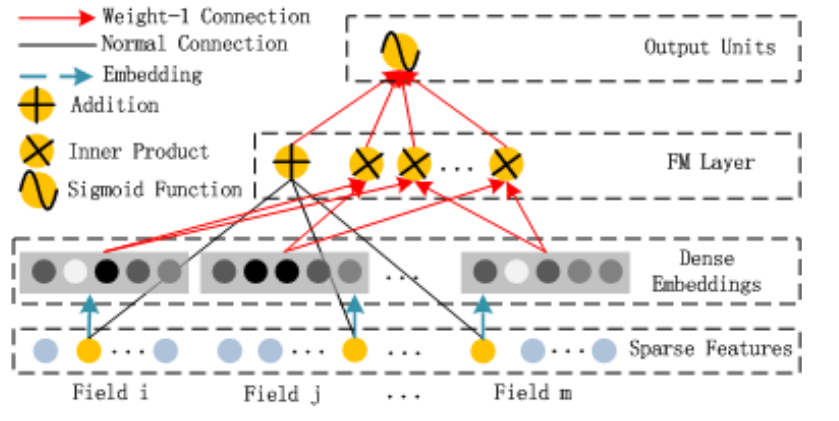
\includegraphics[scale=0.25]{FM_layers}
		\caption{FM layer in DeepFM model}
	\end{figure}
	\[
	y_{out} = \sigma(w_{0} + \sum_{i=1}^{i=n} w_{i} x_{i} + \sum_{i=1}^n \sum_{j=i+1}^n<v_i, v_j>x_i x_j)
	\]
\end{frame}

\begin{frame}
	\frametitle{Deep component}
	Deep component is a feed-forward neural network. \\
	It is used to learn high-order feature interactions. \\
	\begin{figure}
		\includegraphics[scale=0.25]{deep}
		\caption{DNN layer in DeepFM model}
	\end{figure}
\end{frame}

\begin{frame}
	\frametitle{Full DeepFM architecture}
	\begin{figure}
		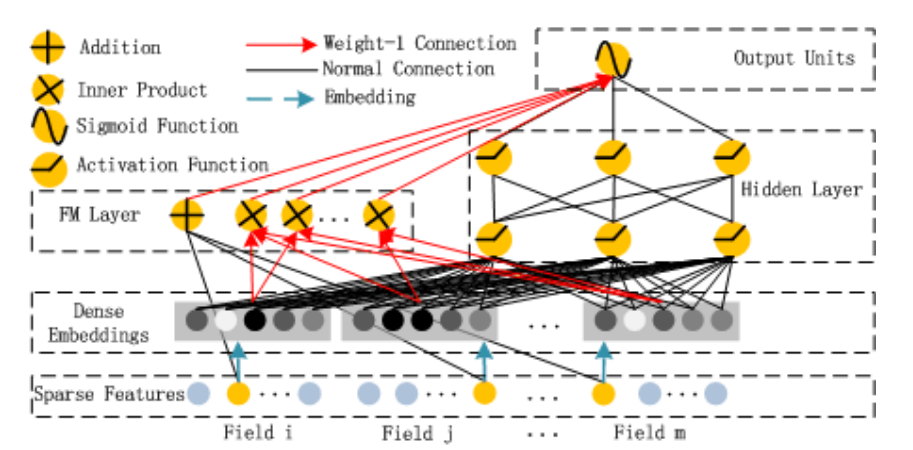
\includegraphics[scale=0.25]{full_deepFM}
		\caption{Wide \& deep architecture of DeepFM.}
	\end{figure}
	Need to add a part same as Wide\& Deep's wide part.
\end{frame}

\begin{frame}
	\frametitle{Full DeepFM architecture}
	\begin{figure}
		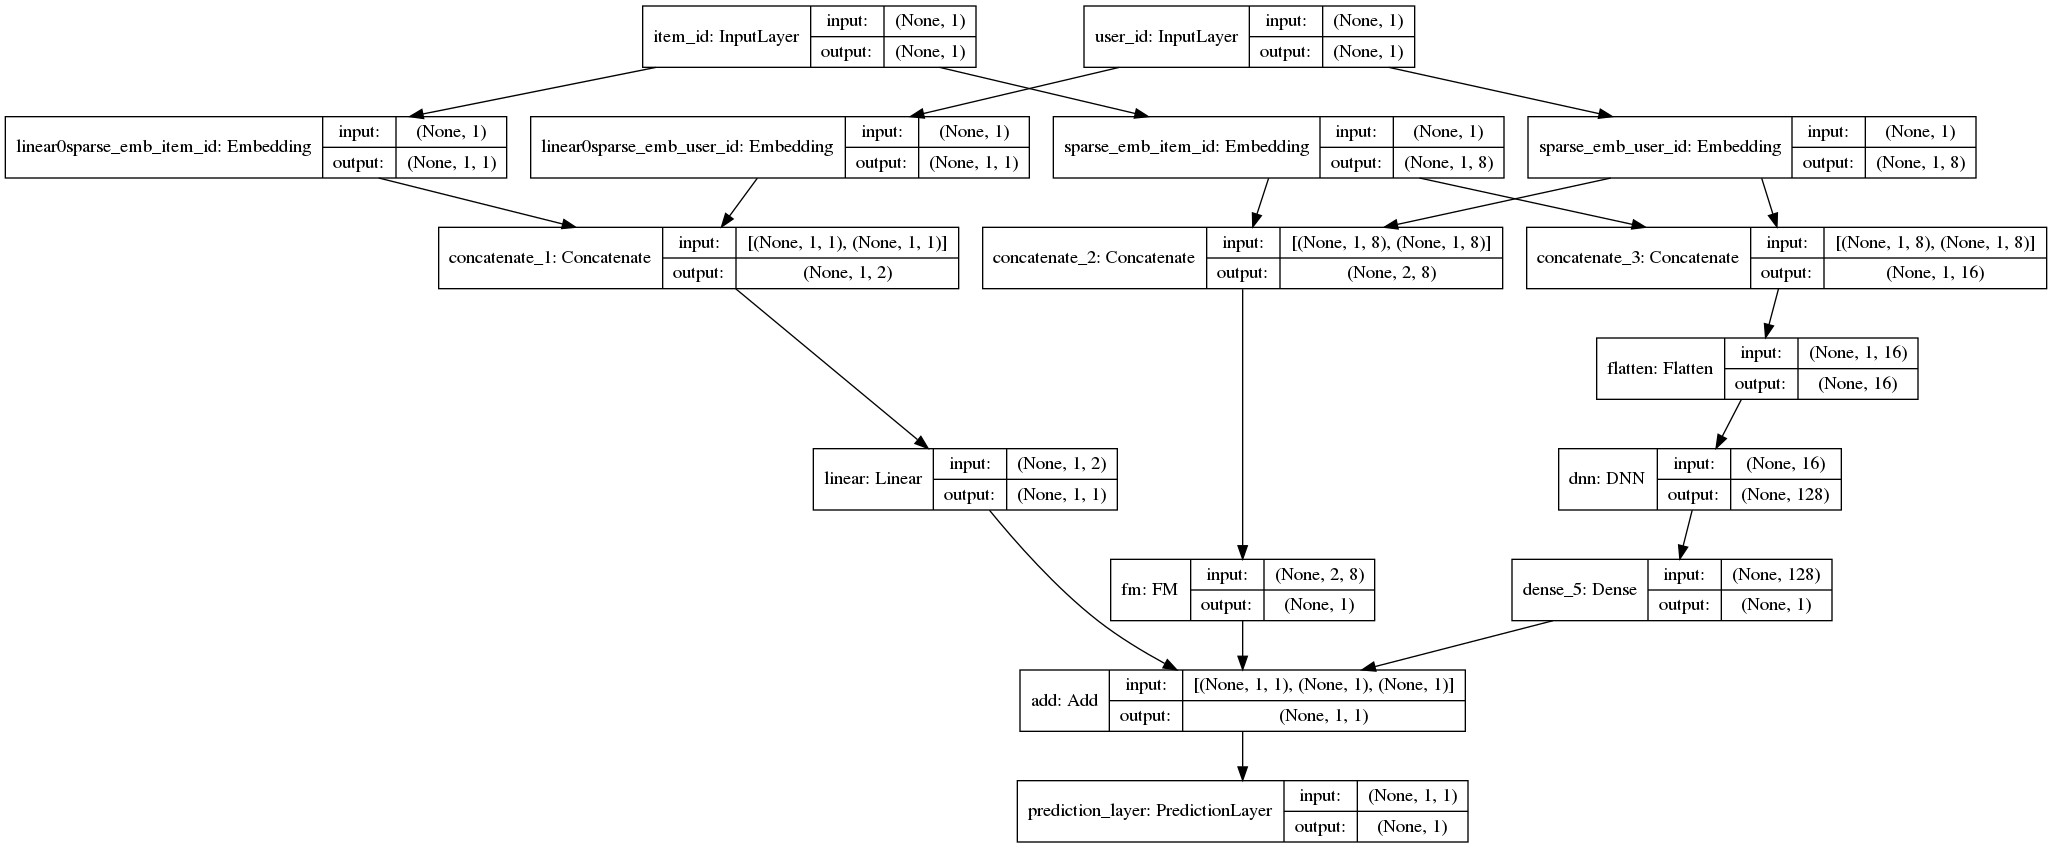
\includegraphics[scale=0.16]{custom_deepFM}
		\caption{Wide \& deep architecture of DeepFM.}
	\end{figure}
\end{frame}

\subsection{Compare to Wide\&Deep}
\begin{frame}
	\frametitle{Wide and deep model}
	\begin{figure}
		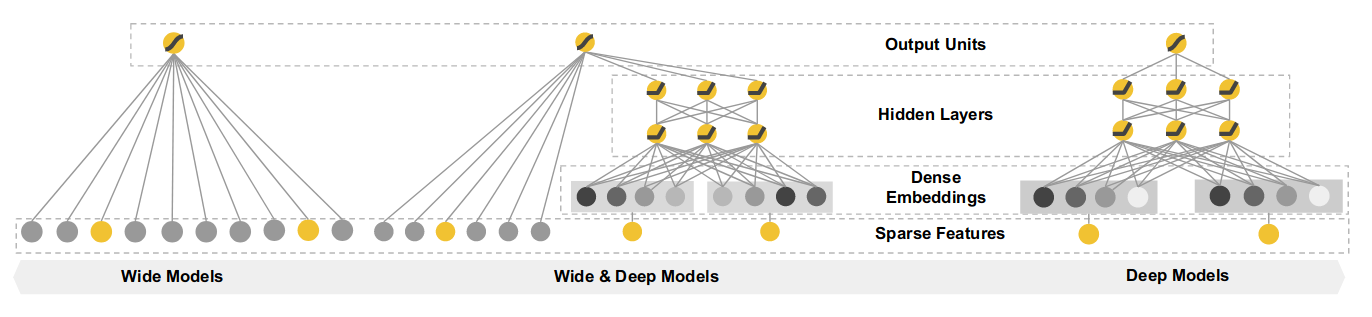
\includegraphics[scale=0.22]{wnd}
		\caption{Wide and Deep model}
	\end{figure}
	
	\begin{itemize}
		\item W\&D can model low and high feature interactions simultaneously. 
		\item It needs for manumal expertise feature engineering on the input. 
		\item W\&D do not generalize to features pairs that have appeared in the training data. 
	\end{itemize}
\end{frame}

\begin{frame}
	\frametitle{Comparison}
	\center{
	\begin{tabular}{|c|c|c|}
		\hline & Wide\& Deep & DeepFM \\
		\hline High-order feature & \checkmark & \checkmark \\
		\hline Low-order feature & \checkmark & \checkmark \\
		\hline No feature engineering & \checkmark & x \\ \hline
	\end{tabular}}
\end{frame}

\begin{frame}
	\frametitle{Experiments}
	\begin{figure}
		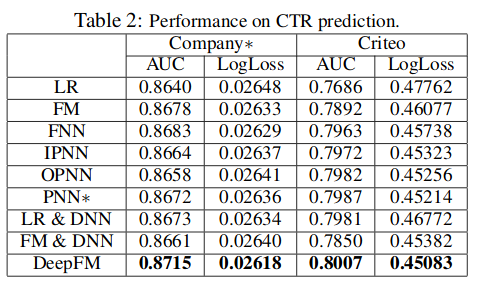
\includegraphics[scale=0.5]{experiment}
	\end{figure}
\end{frame}

\section{References}
\begin{frame}
	\frametitle{References}
	\begin{itemize}
		\item \href{https://www.analyticsvidhya.com/blog/2018/01/factorization-machines/}{Factorization Machines \& their application on huge datasets}
		\item \href{http://berwynzhang.com/2017/01/22/machine_learning/Factorization_Machines/}{Factorization Machine}		
		\item \href{https://www.csie.ntu.edu.tw/~b97053/paper/Rendle2010FM.pdf}{Factorization Machine Paper}
		\item \href{https://arxiv.org/pdf/1703.04247.pdf}{Deep Factorization Machine Paper}
	\end{itemize}
\end{frame}


\end{document}